\documentclass[journal,10pt,twocolumn]{IEEEtran}

\usepackage[utf8]{inputenc}
\usepackage[T1]{fontenc}
\usepackage{amsmath,amssymb,amsfonts}
\usepackage{graphicx}
\usepackage{booktabs}
\usepackage{array}
\usepackage{cite}
\usepackage{url}
\usepackage{microtype}
\usepackage{xcolor}
\usepackage{tabularx}
\usepackage{hyperref}

\hypersetup{
    colorlinks=true,
    linkcolor=black,
    citecolor=black,
    urlcolor=blue
}

\graphicspath{{./}{./figures/}}

\begin{document}

\title{CRISP-DM Phase 2: Data Understanding and Anomaly Taxonomy for Transactional Retail Systems:\\
An Empirical Investigation of North Quay Gifts}

\author{
    \IEEEauthorblockN{
        Russel~Emmanuel~Ku~Aguilar\IEEEauthorrefmark{1},
        Damian~Nicolas~Sanchez~Novelo\IEEEauthorrefmark{1},
        Jonathan~Abisai~Velasco~Mart\'in\IEEEauthorrefmark{1},\\
        \'Angel~Rivaldo~Canch\'e~Chuc\IEEEauthorrefmark{1},
        Bianca~Alexandra~Acosta~Castellanos\IEEEauthorrefmark{1}, and
        Didier~Omar~Gamboa~Angulo\IEEEauthorrefmark{2}
    }\\
    \IEEEauthorblockA{\IEEEauthorrefmark{1}Students, Faculty of Data Engineering, Universidad Polit\'ecnica de Yucat\'an (UPY), M\'erida, Mexico\\
    Email: \{2309131, 2109134, 2309060, 2309030, 2309001\}@upy.edu.mx}\\
    \IEEEauthorblockA{\IEEEauthorrefmark{2}Professor \& Academic Advisor, Faculty of Data Engineering, Universidad Polit\'ecnica de Yucat\'an\\
    Email: didier.gamboa@upy.edu.mx}
}

\maketitle

\begin{abstract}
Under the Cross-Industry Standard Process for Data Mining (CRISP-DM) framework, Phase 2 (Data Understanding) serves as the foundational safeguard against modeling invalidity. This technical report provides a rigorous empirical analysis of the two-year transactional ledger of North Quay Gifts (1,067,371 records from December 2009 to December 2011). We establish a formal anomaly taxonomy that dissects recording mechanics, distributional moments, and structural deficits. Key empirical findings reveal: (i) an extreme leptokurtic distribution in transaction quantities ($\text{Kurtosis} = 155,059.71$) and prices ($\text{Kurtosis} = 73,751.83$), rendering standard parametric moments invalid; (ii) an acute customer missingness rate of 22.77\% (243,007 rows) that necessitates a bifurcated data modeling pipeline; (iii) the definitive empirical distinction between commercial sales returns (prefix `C', 19,494 rows with active pricing) and warehouse inventory shrinkage (3,457 non-`C' negative rows, 100\% characterized by zero price and unassigned customer IDs); and (iv) isolated accounting write-offs (prefix `A', reaching $-\pounds 53,594.36$). Finally, we formulate an actionable, prioritized Data Preparation strategy designed to support Customer Lifetime Value (CLV) and churn prediction without compromising baseline retail demand forecasting.
\end{abstract}

\begin{IEEEkeywords}
CRISP-DM, Data Understanding, Exploratory Data Analysis, E-Commerce Analytics, Anomaly Detection, Reverse Logistics, Customer Lifetime Value (CLV).
\end{IEEEkeywords}

\section{Introduction and Business Context}
\IEEEPARstart{E}{nterprise} machine learning pipelines deployed within direct-to-consumer and business-to-business (B2B) retail environments are exceptionally sensitive to upstream data anomalies \cite{wirth2000crisp}. In the preceding Business Understanding phase (CRISP-DM Phase 1), North Quay Gifts formulated a strategic data science objective: to forecast Customer Lifetime Value (CLV) over a forward-looking horizon of 3 to 6 months while adjusting for individual customer cancellation and return risks \cite{fader2005counting, clv2025forecasting}. However, historical enterprise resource planning (ERP) logs rarely record clean, isolated customer transactions; rather, they serve as heterogeneous capture repositories combining legitimate purchases, wholesale lot allocations, checkout transmission errors, logistical product breakages, and manual accounting reconciliations.

The present investigation executes Phase 2 (Data Understanding) on the complete \textit{Online Retail II} transactional corpus \cite{chen2012online}. Operating under strict governance guidelines—prohibiting premature imputation, arbitrary row deletion, or synthetic feature engineering—we dissect the empirical properties of the ledger. By isolating operational patterns from commercial intent, this study provides the formal empirical baseline required to govern subsequent data preparation and predictive modeling.

\section{Data Recognition and Architectural Semantics}

\subsection{Granularity and Dataset Dimensions}
The raw repository spans 1,067,371 recorded rows across 8 distinct attributes. A critical initial architectural finding concerns the \textit{unit of analysis}: an individual row does not represent an entire purchase order or unique customer visit; rather, it denotes a single merchandise line item within a billing invoice. As summarized in Table~\ref{tab:recognition_indicators}, the corpus encompasses 53,628 unique invoice numbers issued to 5,942 distinct identified customer profiles between December 1, 2009, at 07:45:00 and December 9, 2011, at 12:50:00.

\begin{table}[htbp]
\caption{System Recognition and Global Indicators}
\label{tab:recognition_indicators}
\centering
\begin{tabularx}{\columnwidth}{lX}
\toprule
\textbf{Indicator} & \textbf{Observed Empirical Value} \\
\midrule
Matrix Dimensions & 1,067,371 rows $\times$ 8 columns \\
Temporal Range & 2009-12-01 07:45:00 to 2011-12-09 12:50:00 \\
Distinct Invoices & 53,628 unique transaction identifiers \\
Identified Customers & 5,942 unique accounts (excluding nulls) \\
Atomic Unit of Analysis & Transaction merchandise line item \\
Total Catalog SKUs & 5,305 distinct \texttt{StockCode} entries \\
Geographic Breadth & 43 sovereign trading destinations \\
\bottomrule
\end{tabularx}
\end{table}

\subsection{Analytical Variable Classification}
Rigorous statistical treatment requires classifying attributes according to Stevens' theory of measurement scales \cite{stevens1946theory}. As detailed in Table~\ref{tab:variable_taxonomy}, variables stored as numeric primitives in Pandas do not necessarily represent quantitative scales:

\begin{table*}[htbp]
\caption{Analytical Variable Classification and Schema Taxonomy}
\label{tab:variable_taxonomy}
\centering
\begin{tabularx}{\textwidth}{llllX}
\toprule
\textbf{Attribute} & \textbf{Storage Type} & \textbf{Analytical Scale} & \textbf{Role in Pipeline} & \textbf{Domain Semantics and Behavioral Function} \\
\midrule
\texttt{Invoice} & \texttt{object} (string) & Nominal Identifier & Transaction Key & Alphanumeric order identifier. Prefix `C' denotes cancellation transactions. \\
\texttt{StockCode} & \texttt{object} (string) & Nominal Categorical & Item Key & Alphanumeric SKU. Encompasses physical products and administrative codes. \\
\texttt{Description} & \texttt{object} (string) & Qualitative Textual & Attribute & Commercial title of item, or unstructured internal operational audit note. \\
\texttt{Quantity} & \texttt{int64} & Quantitative Discrete & Metric Scale & Billed physical units. Positive for orders; negative for cancellations/shrinkage. \\
\texttt{InvoiceDate} & \texttt{datetime64[ns]} & Interval Temporal & Temporal Feature & Exact timestamp of order generation. Governs temporal feature extraction. \\
\texttt{Price} & \texttt{float64} & Quantitative Ratio & Metric Scale & Unit selling price in GBP ($\pounds$). Non-positive values represent adjustments. \\
\texttt{Customer ID} & \texttt{float64} & Nominal Identifier & Entity Key & Unique client account key. Stored as float due to IEEE 754 NaN missing values. \\
\texttt{Country} & \texttt{object} (string) & Nominal Categorical & Demographic & Sovereign nation of customer billing/shipping destination. \\
\bottomrule
\end{tabularx}
\end{table*}

\begin{enumerate}
    \item \textbf{Nominal Identifiers as Numeric Primitives:} \texttt{Customer ID} is physically represented as an IEEE-754 \texttt{float64} solely to accommodate missing values (\texttt{NaN}). Computing arithmetic operations such as $\mu(\texttt{Customer ID}) = 15555.57$ yields an analytically meaningless value corresponding to no real entity. Identifiers serve strictly for relational joins and discrete entity tracking.
    \item \textbf{Transaction Granularity Discrepancy:} Analysis of multi-item orders reveals that the number of invoice rows frequently exceeds the number of distinct products. For example, Invoice \texttt{489517} (dated 2009-12-01 11:34:00, Customer 16329.0) contains 38 total rows but only 28 distinct \texttt{StockCode} values. Multiple items (e.g., \texttt{21491}, \texttt{21821}, \texttt{21912}) appear in duplicated rows generated at the identical minute. This occurs when consumers add items across distinct basket-building iterations or when point-of-sale systems fail to aggregate repeated line inputs. Equating transaction rows to orders would artificially inflate sales frequency by a factor of $19.9\times$.
    \item \textbf{Temporal Truncation Bias:} Examining boundary months reveals incomplete coverage. December 2009 records 45,228 rows spanning 21 active trading days (terminating abruptly on December 23), missing the post-Christmas liquidation cycle. December 2011 terminates on December 9 at 12:50:00, containing only 25,526 rows across 8 days (compared to 84,711 rows in November 2011). Unadjusted period-over-period aggregate comparisons between 2010 and 2011 would introduce severe artificial contraction bias.
\end{enumerate}

\section{Descriptive Statistics and Distributional Moments}

\subsection{Central Tendency and Non-Parametric Dispersion}
Parametric estimation based on sample mean and standard deviation fails when analyzing unconstrained retail transaction streams. Table~\ref{tab:desc_stats} contrasts parametric and non-parametric summary metrics for \texttt{Quantity} and \texttt{Price}.

\begin{table}[htbp]
\caption{Distributional Moments and Descriptive Statistics}
\label{tab:desc_stats}
\centering
\begin{tabularx}{\columnwidth}{Xrr}
\toprule
\textbf{Descriptive Statistic} & \textbf{Quantity (Units)} & \textbf{Price ($\pounds$ GBP / Unit)} \\
\midrule
Valid Observations ($N$) & 1,067,371 & 1,067,371 \\
Mean ($\mu$) & 9.9389 & 4.6494 \\
Median ($Q_2$) & 3.0000 & 2.1000 \\
Standard Deviation ($\sigma$) & 172.7058 & 123.5531 \\
Minimum & $-80,995$ & $-\pounds 53,594.36$ \\
Lower Quartile ($Q_1$ - 25\%) & 1.0000 & $\pounds 1.2500$ \\
Upper Quartile ($Q_3$ - 75\%) & 10.0000 & $\pounds 4.1500$ \\
Maximum & $+80,995$ & $+\pounds 38,970.00$ \\
Skewness ($\gamma_1$) & $+3.9961$ & $-69.1647$ \\
Fisher Excess Kurtosis ($\gamma_2$) & $+155,059.71$ & $+73,751.83$ \\
\bottomrule
\end{tabularx}
\end{table}

For \texttt{Quantity}, the sample mean ($\mu = 9.94$) is more than three times the median ($Q_2 = 3.00$), driven by massive positive wholesale orders of up to 80,995 units. The interquartile range ($\text{IQR} = Q_3 - Q_1 = 9.00$) reveals that 50\% of all transaction lines involve between 1 and 10 items. For \texttt{Price}, the median is $\pounds 2.10$ ($\text{IQR} = \pounds 2.90$), whereas the mean ($\pounds 4.65$) is heavily influenced by massive accounting adjustments and administrative service fees.

The Fisher excess kurtosis values ($\gamma_2 = 155,059.71$ for \texttt{Quantity} and $\gamma_2 = 73,751.83$ for \texttt{Price}) represent extreme heavy-tailed leptokurtosis. The negative price skewness ($\gamma_1 = -69.16$) is directly attributable to isolated bad-debt write-offs exceeding $-\pounds 53,000$. Consequently, the sample mean cannot be reported as an indicator of a ``typical'' customer purchase without introducing profound modeling errors.

\subsection{Categorical Dispersion: Geographic vs. Catalog Entropy}
Analysis of categorical distributions reveals a sharp dichotomy between extreme geographic concentration and massive product catalog entropy (Table~\ref{tab:cat_summary}).

\begin{table}[htbp]
\caption{Categorical Diversity and Modal Concentration}
\label{tab:cat_summary}
\centering
\begin{tabularx}{\columnwidth}{lrrrX}
\toprule
\textbf{Variable} & \textbf{Valid} & \textbf{Unique} & \textbf{Modal SKU/Nation} & \textbf{Modal Share} \\
\midrule
\texttt{Country} & 1,067,371 & 43 & United Kingdom & 981,330 (91.94\%) \\
\texttt{StockCode} & 1,067,371 & 5,305 & 85123A & 5,829 (0.55\%) \\
\bottomrule
\end{tabularx}
\end{table}

As illustrated in Table~\ref{tab:top3_categories}, the United Kingdom accounts for 91.94\% of all ledger lines, with the top 10 countries collectively representing 98.46\% (1,050,946 lines). In contrast, the merchandise catalog exhibits high dispersion across 5,305 unique SKUs. The single most frequent product (\texttt{85123A}, \textit{White Hanging Heart T-Light Holder}) captures only 0.55\% of transaction volume, and the top 10 SKUs combined encompass just 3.24\% of all lines (34,610 lines).

\begin{table}[htbp]
\caption{Three Most Frequent Categories and Line Shares}
\label{tab:top3_categories}
\centering
\begin{tabularx}{\columnwidth}{lX}
\toprule
\textbf{Variable} & \textbf{Top 3 Categories with Line Count and Total Share} \\
\midrule
\texttt{Country} & 1. \textbf{United Kingdom}: 981,330 lines (91.94\%) \\
& 2. \textbf{EIRE}: 17,866 lines (1.67\%) \\
& 3. \textbf{Germany}: 17,624 lines (1.65\%) \\
\midrule
\texttt{StockCode} & 1. \textbf{85123A} (Heart T-Light): 5,829 lines (0.55\%) \\
& 2. \textbf{22423} (Cakestand 3 Tier): 4,424 lines (0.41\%) \\
& 3. \textbf{85099B} (Jumbo Bag Retrospot): 4,216 lines (0.39\%) \\
\bottomrule
\end{tabularx}
\end{table}

A crucial business insight emerges: transaction line frequency does not correlate directly with order volume, unit sales, or gross profitability. A low-cost novelty souvenir item (e.g., a $\pounds 0.42$ trinket) may appear across thousands of separate orders as a single-unit basket addition, while a high-value home furnishing item (e.g., a $\pounds 12.75$ tiered stand) generates far higher monetary revenue with fewer invoice lines.

\section{Univariate Analysis and Outlier Detection}

\subsection{Empirical Distribution and Window Truncation}
Because extreme values compress standard histograms into single-bin spikes, we evaluate both full-range log-scaled distributions and high-density bounded windows.

\begin{figure}[htbp]
\centering
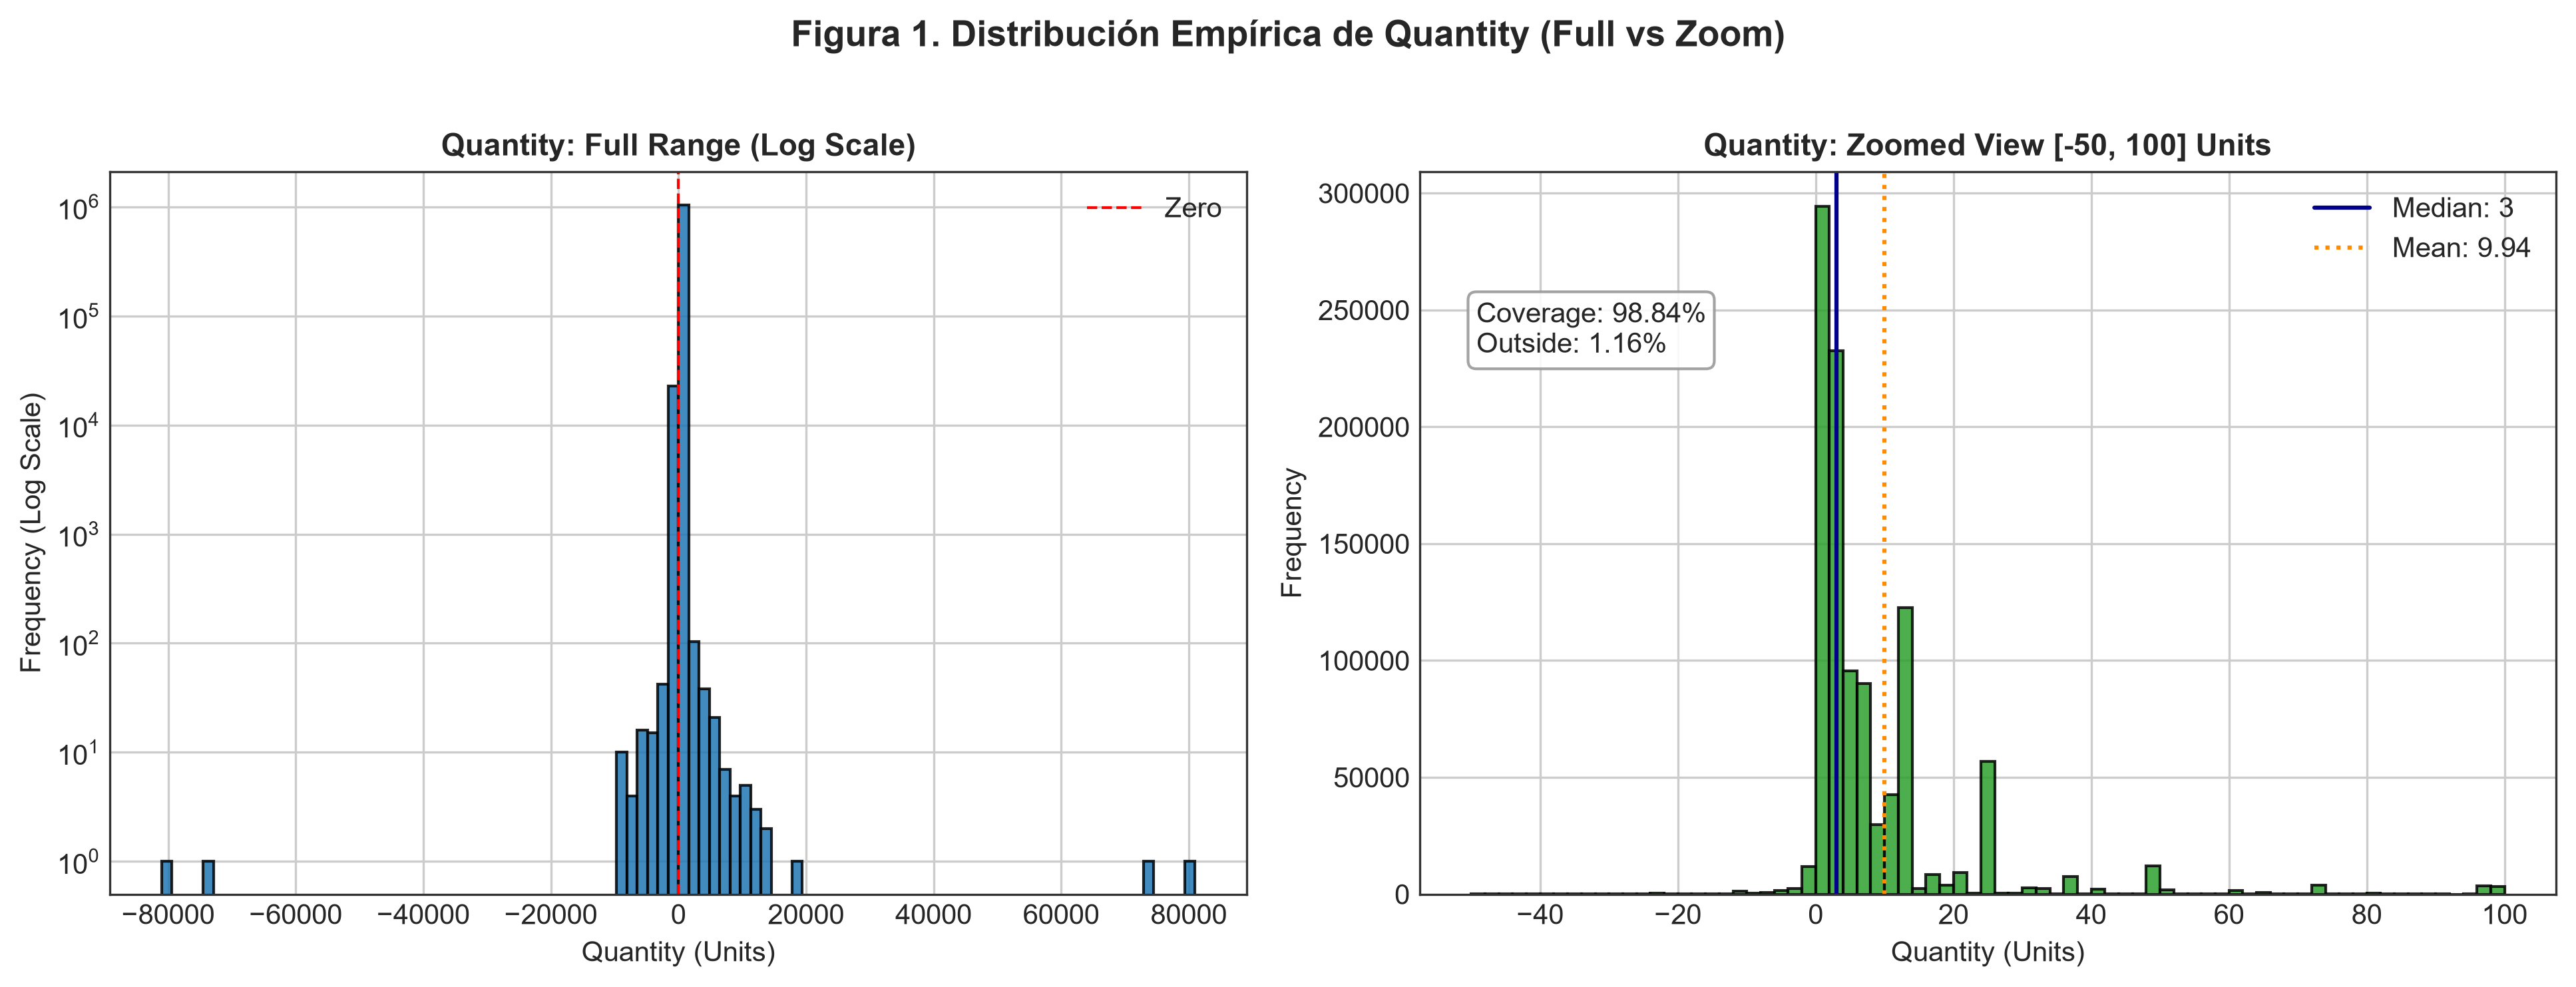
\includegraphics[width=\columnwidth]{figures/fig1_quantity_hist.png}
\caption{Empirical distribution of \texttt{Quantity}. Left: Full range on a logarithmic frequency scale demonstrating extreme symmetric tails ($\pm 80,995$). Right: Focused window $[-50, 100]$ capturing 98.84\% of observations, highlighting modal concentration at 1–3 units.}
\label{fig:quantity_hist}
\end{figure}

\begin{figure}[htbp]
\centering
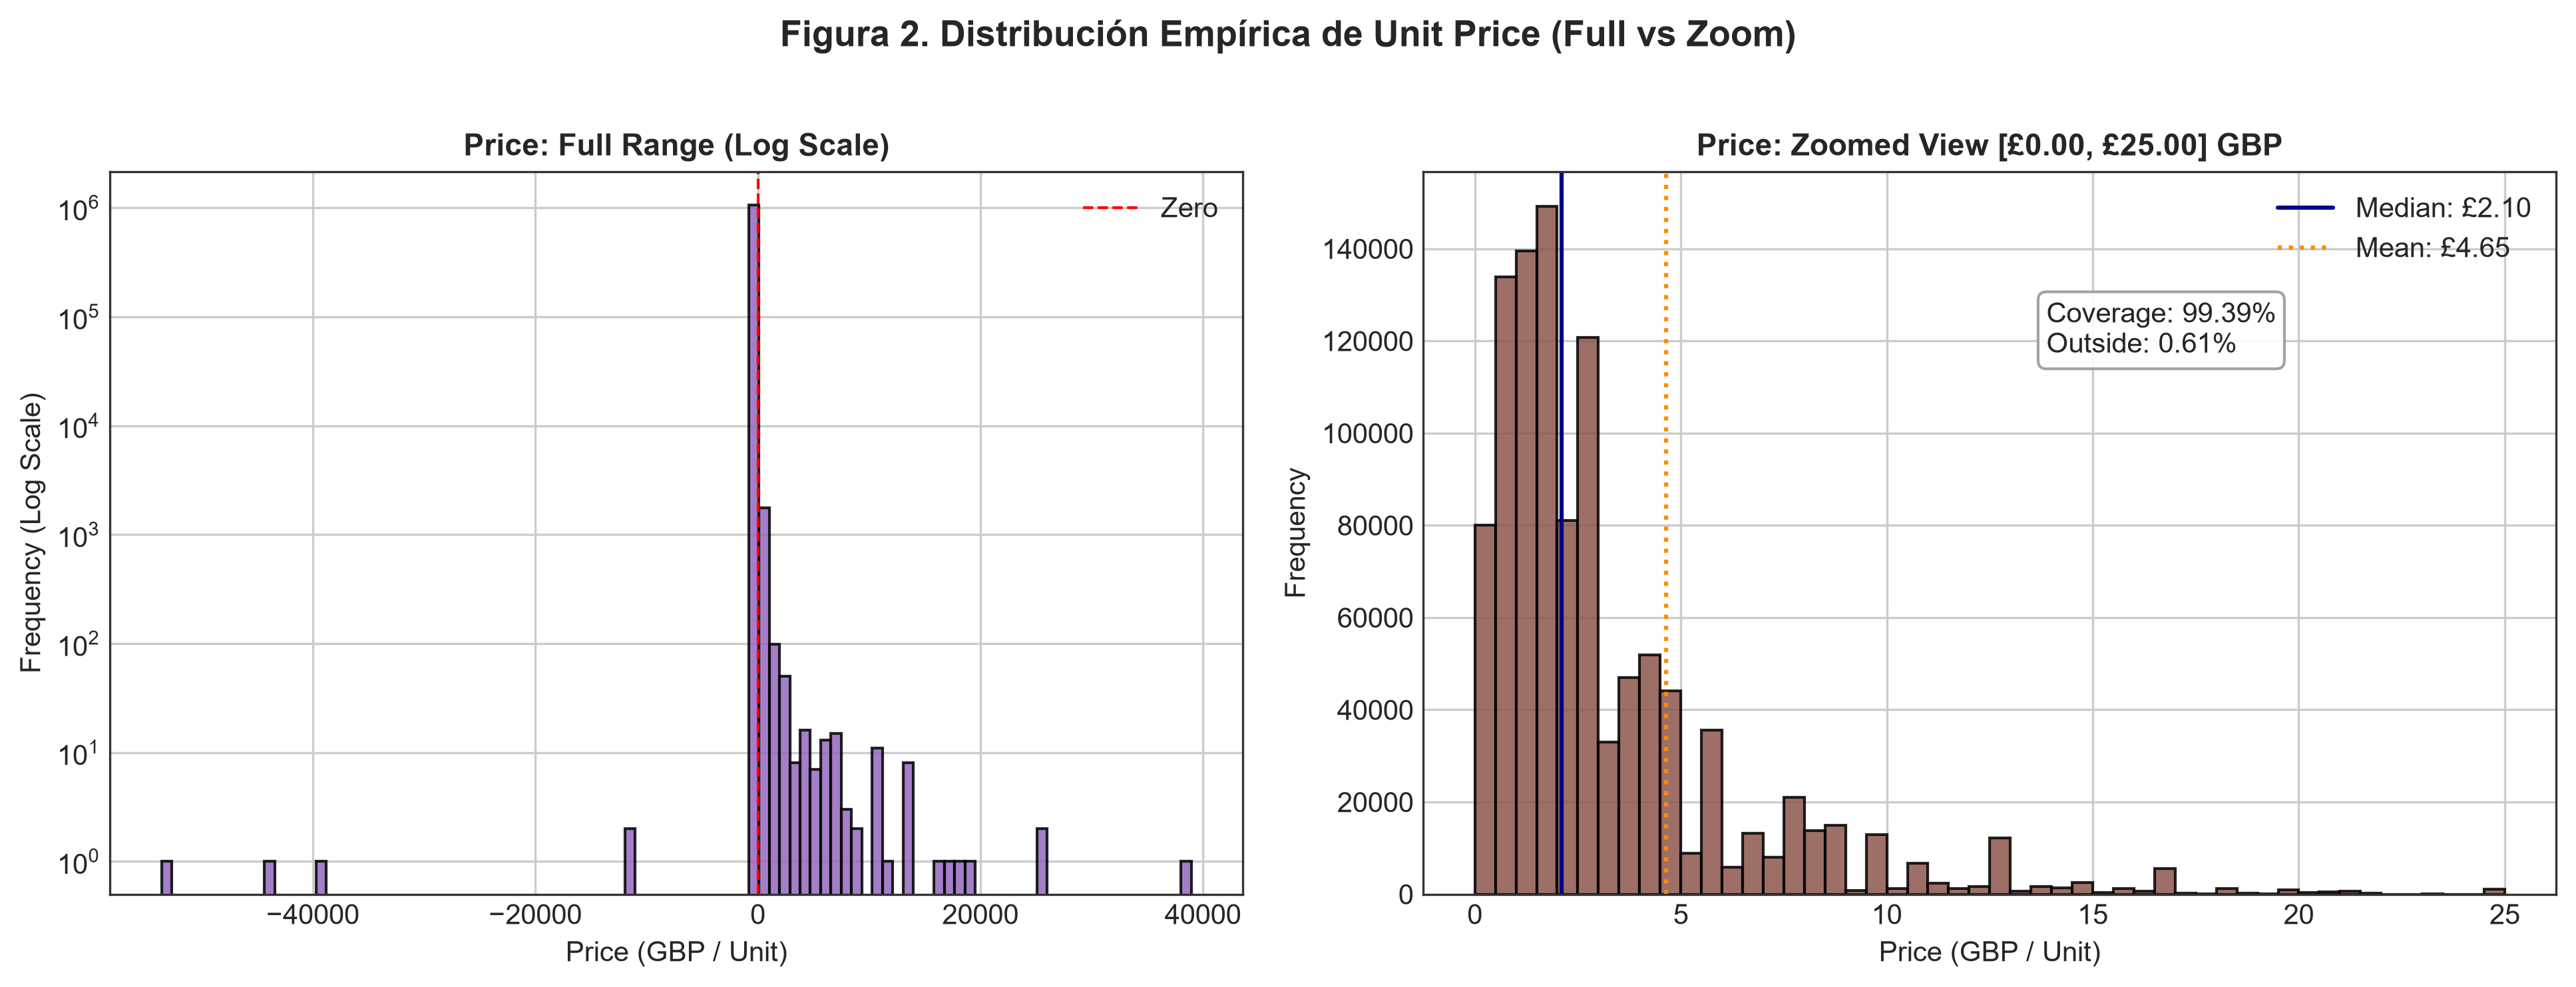
\includegraphics[width=\columnwidth]{figures/fig2_price_hist.png}
\caption{Empirical distribution of unit \texttt{Price}. Left: Full range log-scaled histogram illustrating positive fee outliers and isolated negative accounting entries. Right: High-density window $[\pounds 0.00, \pounds 25.00]$ enclosing 99.39\% of transaction lines.}
\label{fig:price_hist}
\end{figure}

As depicted in Fig.~\ref{fig:quantity_hist}, restricting the observation window of \texttt{Quantity} to $[-50, 100]$ units captures 98.84\% of all recorded transactions, leaving only 1.16\% outside the boundaries. In this core domain, over 95.53\% of positive purchases involve between 1 and 50 units. 

Similarly, for unit \texttt{Price} (Fig.~\ref{fig:price_hist}), constraining the visual window to $[\pounds 0.00, \pounds 25.00]$ encloses 99.39\% of all transaction lines (with only 0.61\% lying outside). Over 98.17\% of retail merchandise is priced between $\pounds 0.00$ and $\pounds 15.00$, exhibiting sharp modal density at $\pounds 1.25$, $\pounds 1.65$, and $\pounds 2.10$.

\begin{figure}[htbp]
\centering
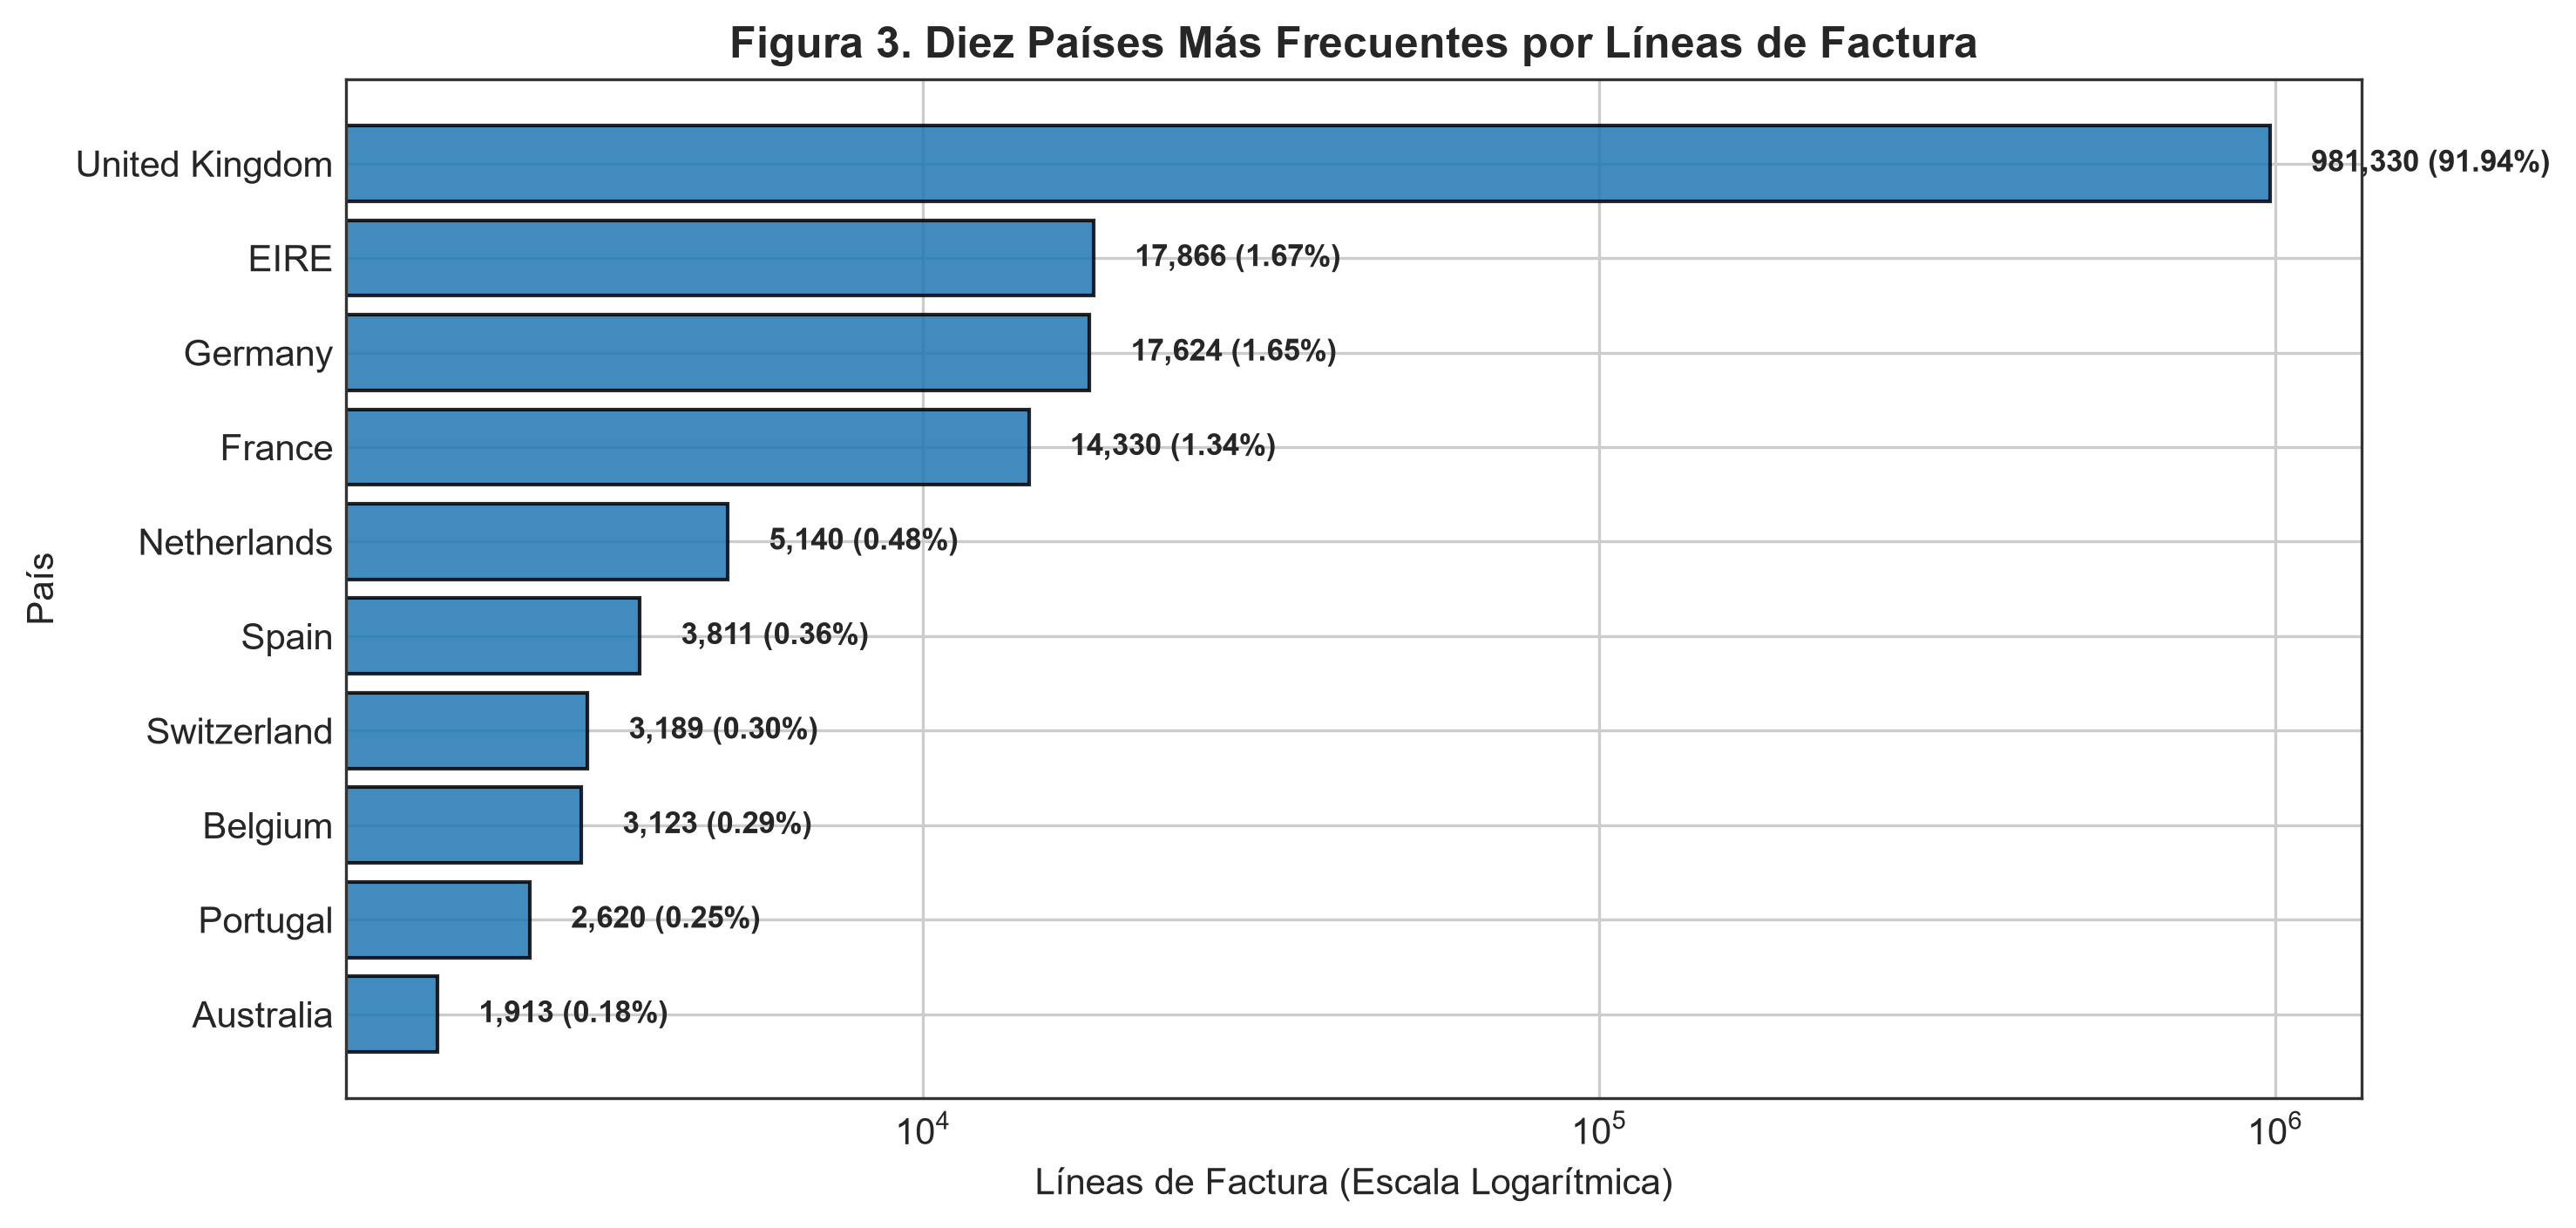
\includegraphics[width=\columnwidth]{figures/fig3_country_bar.png}
\caption{Log-scaled frequency distribution of the top 10 sovereign destinations, emphasizing the domestic UK market dominance alongside secondary European hubs.}
\label{fig:country_bar}
\end{figure}

\begin{figure}[htbp]
\centering
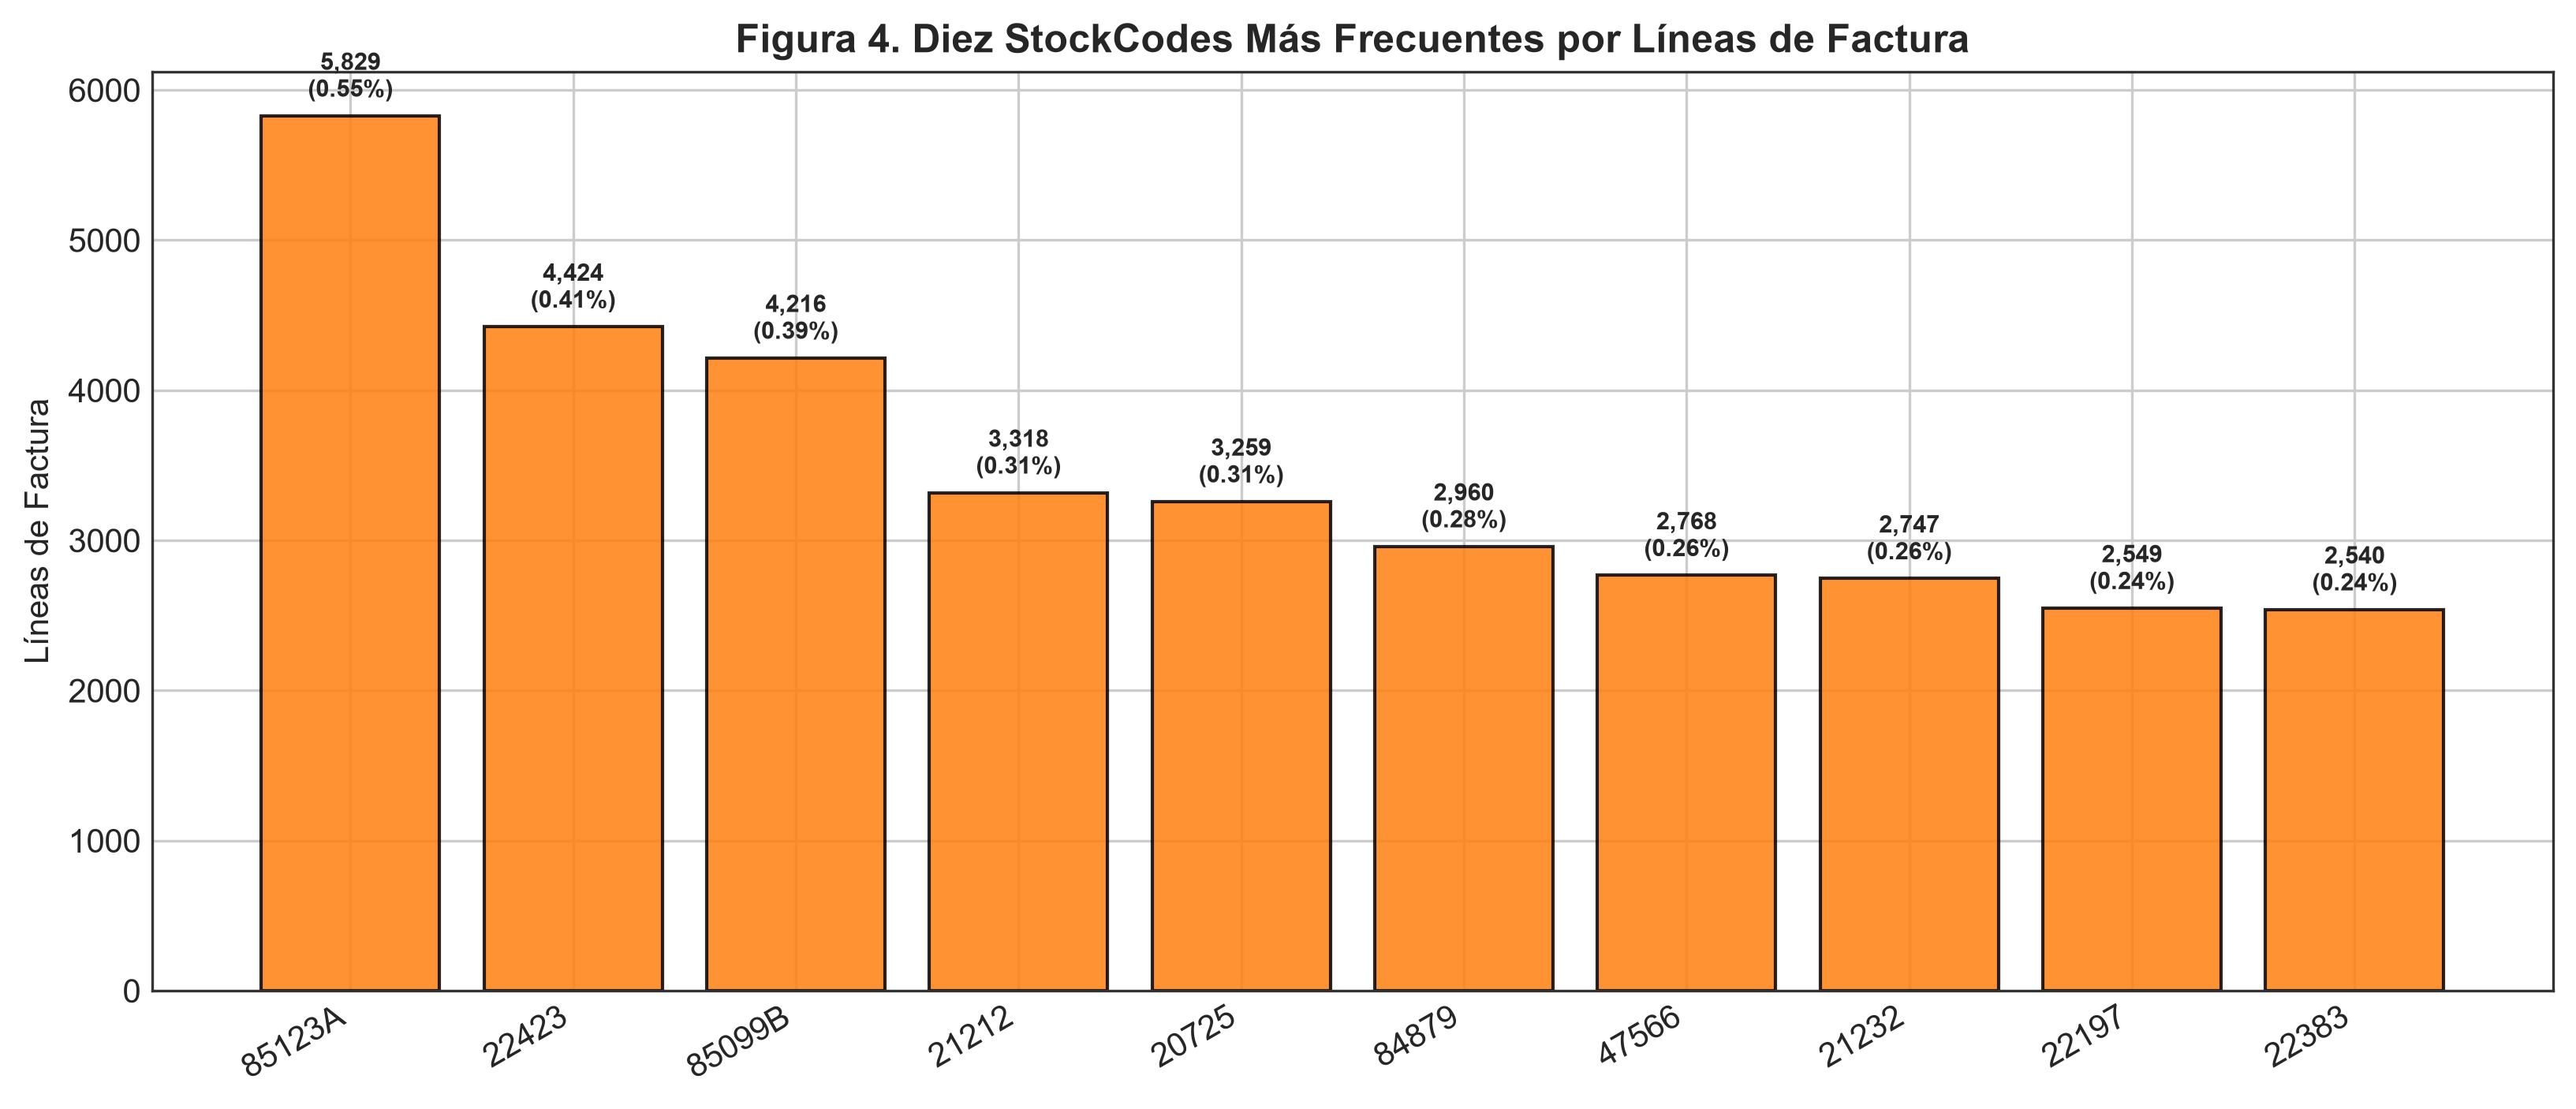
\includegraphics[width=\columnwidth]{figures/fig4_stockcode_bar.png}
\caption{Frequencies of the top 10 merchandise SKUs, confirming extensive catalog dispersion where the leading item captures barely 0.55\% of rows.}
\label{fig:stockcode_bar}
\end{figure}

\subsection{Tukey Boxplot Analysis and Outlier Taxonomy}
Outlier detection was formalized using Tukey's non-parametric fence rule \cite{tukey1977exploratory}, where inner fences are located at:
\begin{equation}
\text{Lower Whisker} = \max\left(\min(X), Q_1 - 1.5 \times \text{IQR}\right)
\end{equation}
\begin{equation}
\text{Upper Whisker} = \min\left(\max(X), Q_3 + 1.5 \times \text{IQR}\right)
\end{equation}

For \texttt{Quantity}, with $Q_1 = 1.0$ and $Q_3 = 10.0$ ($\text{IQR} = 9.0$), the mathematical upper whisker terminates at $10.0 + 1.5(9.0) = 23.5$ units (Fig.~\ref{fig:boxplots}). In standard retail analytics, classifying every transaction exceeding 24 units as an ``error'' would be catastrophic: North Quay operates a dual retail-wholesale commercial model, where genuine wholesale clients routinely order 100 to 500 units in commercial lots.

\begin{figure}[htbp]
\centering
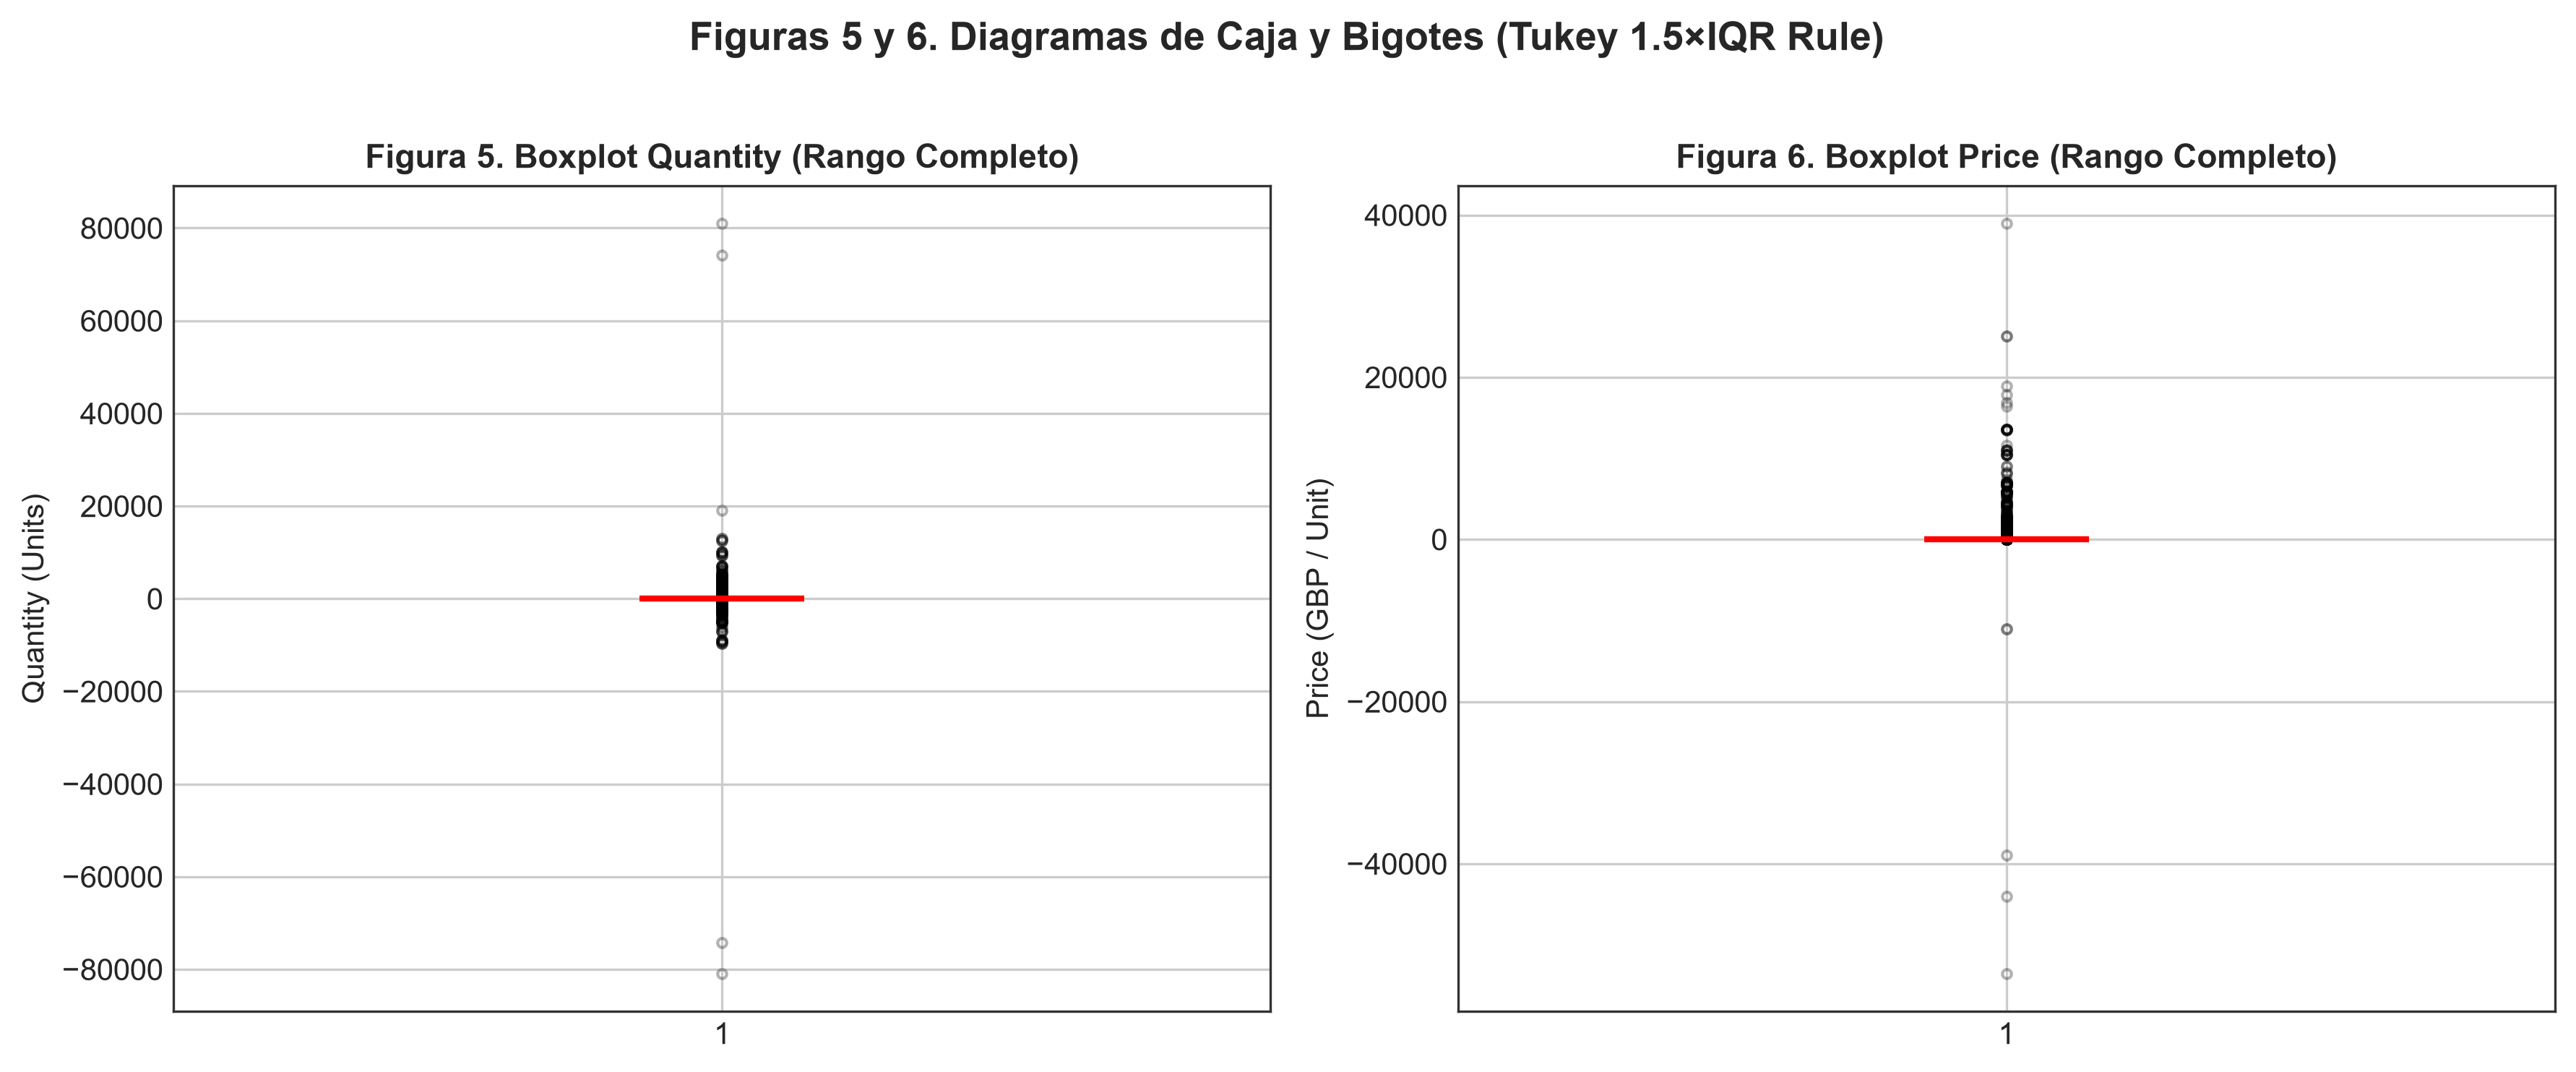
\includegraphics[width=\columnwidth]{figures/fig5_6_boxplots.png}
\caption{Boxplots for \texttt{Quantity} (left) and unit \texttt{Price} (right) constructed under Tukey's $1.5 \times \text{IQR}$ rule, demonstrating severe outlier dispersion.}
\label{fig:boxplots}
\end{figure}

A mathematical outlier cannot be conflated with corrupted data. Genuine bulk orders are characterized by valid commercial prices, existing customer IDs, and normal product descriptions. Conversely, true errors exhibit contextual anomalies—such as null customer accounts, negative unit prices, or administrative adjustment labels.

\section{Data Quality Diagnostics}

\subsection{Completeness Audit with Homogeneous Denominators}
To evaluate data cleanliness, null counts across all eight columns were evaluated using a single homogeneous denominator ($N = 1,067,371$), as presented in Table~\ref{tab:null_diagnostics}.

\begin{table}[htbp]
\caption{Completeness and Null Value Diagnostic Matrix}
\label{tab:null_diagnostics}
\centering
\begin{tabularx}{\columnwidth}{Xrr}
\toprule
\textbf{Column Attribute} & \textbf{Null Count} & \textbf{Percentage of Total ($N = 1,067,371$)} \\
\midrule
\texttt{Invoice} & 0 & 0.0000\% \\
\texttt{StockCode} & 0 & 0.0000\% \\
\texttt{Description} & 4,382 & 0.4105\% \\
\texttt{Quantity} & 0 & 0.0000\% \\
\texttt{InvoiceDate} & 0 & 0.0000\% \\
\texttt{Price} & 0 & 0.0000\% \\
\texttt{Customer ID} & 243,007 & 22.7669\% \\
\texttt{Country} & 0 & 0.0000\% \\
\bottomrule
\end{tabularx}
\end{table}

\texttt{Customer ID} exhibits a deficit of 243,007 rows (22.77\%). This structural missingness establishes an analytical barrier: individual-level RFM metrics (Recency, Frequency, Monetary value), CLV models, and churn probabilities cannot be computed for anonymous buyers. However, these identical records remain essential for macro-commercial planning: they capture legitimate walk-in and guest retail revenues, inventory depletion, and aggregate seasonal demand.

\subsection{Exact Duplicates and Transmission Errors}
Execution of \texttt{df.duplicated()} across all eight original columns identified 34,335 additional exact duplicate lines (3.22\% of the dataset), as summarized in Table~\ref{tab:situations_table}.

\begin{table}[htbp]
\caption{Prevalence of Anomalous Ledger Records}
\label{tab:situations_table}
\centering
\begin{tabularx}{\columnwidth}{Xrr}
\toprule
\textbf{Anomalous Ledger Situation} & \textbf{Line Count} & \textbf{Percentage of Total} \\
\midrule
Exact Additional Duplicates & 34,335 & 3.2168\% \\
Negative Quantities ($\texttt{Quantity} < 0$) & 22,950 & 2.1501\% \\
Zero Quantity ($\texttt{Quantity} = 0$) & 0 & 0.0000\% \\
Negative Price ($\texttt{Price} < 0$) & 5 & 0.0005\% \\
Zero Price ($\texttt{Price} = 0$) & 6,202 & 0.5811\% \\
\bottomrule
\end{tabularx}
\end{table}

Forensic inspection reveals that these duplicates are not random clerical slips. In Invoice \texttt{489517}, identical SKU lines (e.g., StockCode \texttt{21491}, 6 units at $\pounds 0.65$, Customer 16329.0) appear repeatedly with identical second-level timestamps. This pattern points to checkout payment gateway retries, browser multi-clicks, or ERP message queue re-transmissions. If retained without deduplication, revenue and physical unit demand would be artificially inflated by 3.22\%.

\subsection{Non-Positive Pricing and Accounting Injections}
The ledger contains five records with negative prices ($\texttt{Price} < 0$), all possessing invoice prefix `A' (e.g., \texttt{A506401}, \texttt{A516228}), StockCode \texttt{B}, Quantity 1, null \texttt{Customer ID}, and description \textit{``Adjust bad debt''}. The magnitudes are extreme: $-\pounds 53,594.36$, $-\pounds 44,031.79$, $-\pounds 38,925.87$, and two entries of $-\pounds 11,062.06$. These represent corporate financial adjustments for uncollectible credit balances. If treated as retail sales, they distort gross revenues by $-\pounds 158,676.14$.

Furthermore, 6,202 records feature $\texttt{Price} = \pounds 0.00$. Of these, 6,131 (98.85\%) lack a customer ID and contain internal logistical memos: \textit{``check''} (162 lines), \textit{``damages''} (84 lines), \textit{``damaged''} (81 lines), and \textit{``found''} (28 lines). Only 71 zero-price rows contain identified customer IDs, representing promotional samples or customer compensation items.

\section{Forensic Investigation of Cancellations and Negative Quantities}

\subsection{Taxonomy of Invoice Prefix `C'}
Conventional retail pipelines frequently assume that all negative quantities denote customer cancellations, and conversely, that all cancellations are flagged with prefix `C'. Empirical verification disproves both assumptions.

Analyzing rows with prefix `C' via \texttt{str.startswith('C')} reveals 19,494 lines distributed across 8,292 distinct invoice entities (Table~\ref{tab:c_investigation}). Exactly 19,493 of these lines have $\texttt{Quantity} < 0$, accompanied by active prices and identified customers. 

\begin{table}[htbp]
\caption{Empirical Audit of Invoices with Prefix `C'}
\label{tab:c_investigation}
\centering
\begin{tabularx}{\columnwidth}{Xr}
\toprule
\textbf{Audit Indicator} & \textbf{Empirical Result} \\
\midrule
Total Lines with Prefix `C' & 19,494 lines \\
Distinct Invoice Identifiers (`C') & 8,292 unique orders \\
`C' Lines with $\texttt{Quantity} < 0$ & 19,493 lines \\
`C' Lines with $\texttt{Quantity} = 0$ & 0 lines \\
`C' Lines with $\texttt{Quantity} > 0$ & 1 anomalous line \\
\bottomrule
\end{tabularx}
\end{table}

However, an anomaly exists: exactly one record exhibits prefix `C' alongside a \textit{positive} quantity: Invoice \texttt{C496350}, StockCode \texttt{M} (\textit{``Manual''}), Quantity $+1$, Unit Price $\pounds 373.57$, Customer ID null. Rather than a merchandise return, this represents an administrative billing correction or manual service fee entered under a cancellation invoice number.

\subsection{Negative Quantities without Prefix `C': Warehouse Shrinkage}
A substantial subpopulation consists of negative quantities issued under numeric invoice numbers lacking the `C' prefix: exactly 3,457 lines across 3,393 unique orders.

Empirical evaluation reveals three defining attributes:
\begin{itemize}
    \item \textbf{100\% Zero Price:} All 3,457 lines have $\texttt{Price} = \pounds 0.00$.
    \item \textbf{100\% Missing Customer IDs:} Exactly zero records possess an identified customer account.
    \item \textbf{Logistical Textual Memos:} The descriptions explicitly record operational stock loss: \textit{``check''} (123 lines), \textit{``damages''} (84 lines), \textit{``?''} (83 lines), \textit{``damaged''} (78 lines), \textit{``missing''} (27 lines), \textit{``smashed''} (9 lines), and \textit{``thrown away''} (9 lines).
\end{itemize}

These records do not represent customer product returns; they document internal warehouse inventory write-offs, physical breakage, and cycle-count reconciliations. Conflating these rows with customer returns would severely corrupt return-rate predictive models \cite{returns2015predicting}.

\subsection{Contingency Matrix Cross-Tabulation}
To prove the structural non-equivalence between invoice prefixes and quantity signs, we constructed a complete $2 \times 3$ contingency matrix across the entire 1,067,371-row corpus (Table~\ref{tab:contingency_matrix}).

\begin{table}[htbp]
\caption{Bivariate Contingency Matrix: Invoice Prefix vs. Quantity Sign}
\label{tab:contingency_matrix}
\centering
\begin{tabularx}{\columnwidth}{Xrrr}
\toprule
\textbf{Invoice Prefix} & $\mathbf{Q < 0}$ & $\mathbf{Q = 0}$ & $\mathbf{Q > 0}$ \\
\midrule
With Prefix `C' & 19,493 & 0 & 1 \\
Without Prefix `C' & 3,457 & 0 & 1,044,420 \\
\midrule
\textbf{Total Column} & \textbf{22,950} & \textbf{0} & \textbf{1,044,421} \\
\bottomrule
\end{tabularx}
\end{table}

The empirical evidence demonstrates that prefix `C' lines do not match negative quantities: 15.06\% of all negative records (3,457 of 22,950) originate outside the cancellation series. Treating all negative quantities as a single commercial construct would introduce systematic bias into churn and return propensity algorithms.

\section{Strategic Data Preparation Action Plan}

\subsection{Action Plan and Treatment Matrix}
Based on these diagnostics, we formalize a structured treatment matrix for Phase 3 (Data Preparation), presented in Table~\ref{tab:action_plan}.

\begin{table*}[htbp]
\caption{Strategic Action Plan and Data Preparation Treatment Matrix}
\label{tab:action_plan}
\centering
\begin{tabularx}{\textwidth}{p{2.8cm}p{2.8cm}p{4.0cm}X}
\toprule
\textbf{Identified Anomaly} & \textbf{Empirical Evidence} & \textbf{Potential Business \& Modeling Impact} & \textbf{Proposed Preparation Treatment} \\
\midrule
Missing Customer IDs & 243,007 lines (22.77\%); e.g., Invoice 489435. & Fatal bias in CLV and customer-level RFM; dropping lines discards 22.8\% of cash flow. & \textbf{Bifurcated Pipeline Architecture:} Isolate complete accounts for CLV/churn modeling; retain anonymous lines in an aggregate inventory demand baseline. \\
\midrule
Exact Additional Duplicates & 34,335 lines (3.22\%); e.g., Invoice 489517 identical lines at 11:34:00. & Artificial inflation of unit demand, order frequency, and sales revenues by 3.22\%. & Deduplicate via \texttt{drop\_duplicates(keep='first')}. Audit e-commerce gateway for retry payload handling. \\
\midrule
Negative Quantities without Prefix `C' & 3,457 lines (0.32\%); 100\% $\texttt{Price} = 0$, 100\% missing ID; ``damages'', ``check''. & Conflates warehouse stock breakage with commercial customer churn and return rates. & \textbf{Operational Segregation:} Route directly to an internal Warehouse Shrinkage audit model; purge from customer sales pipelines. \\
\midrule
Non-Positive Prices ($\texttt{Price} \le 0$) & 5 negative lines (`A' prefix, Bad debt up to $-\pounds 53,594.36$); 6,202 zero-price lines. & Severe revenue corruption; bad debt erases hundreds of thousands in gross revenue. & Exclude bad-debt write-offs permanently from commercial sales. Audit zero-price entries for promotional marketing vs logging omissions. \\
\midrule
Commercial Cancellations (Prefix `C') & 19,494 lines (1.83\%); 19,493 $Q < 0$ and 1 anomalous $Q > 0$ (\texttt{C496350}, Manual). & Overstates gross customer revenue if returns are unlinked to original purchase events. & Conciliate returns with original purchase invoices to calculate true net revenue and individual customer return propensities. \\
\midrule
Non-Product Administrative SKUs & 1,983 \texttt{POST}, 214 \texttt{D}, 939 \texttt{M}, 110 \texttt{BANK CHARGES} entries. & Skews product affinity rules, market basket cross-selling, and SKU demand forecasting. & Isolate fee and freight surcharges into dedicated fee vectors; exclude from product recommendation matrices. \\
\bottomrule
\end{tabularx}
\end{table*}

\subsection{Preparation Priority and Residual Risk Assessment}
The most urgent preparation priority is the \textbf{bifurcation of customer records and the exclusion of non-positive prices}. Attempting to train customer lifetime value (CLV) or churn models on anonymous purchases (22.77\% of lines) corrupts customer-level behavioral profiles, while bad-debt accounting write-offs ($-\pounds 53,594.36$ in Invoice \texttt{A506401}) distort revenue scaling. Splitting the pipeline ensures that CRM models receive clean customer histories, while retail inventory demand forecasting retains the complete transaction stream.

However, even after executing this preparation protocol, a critical \textbf{residual risk persists}: unobserved B2B wholesale transaction dynamics. The remaining customer dataset contains wholesale buyers purchasing hundreds of units whose irregular ordering cycles can overwhelm predictive retail models. Without product profit margins, customer acquisition costs, or demographic data, predictive models remain vulnerable to sudden wholesale purchasing shifts.

\section{Conclusion}
This investigation completes the CRISP-DM Phase 2 (Data Understanding) requirements for North Quay Gifts. Through rigorous empirical exploration of 1,067,371 transaction records, we have established:
\begin{enumerate}
    \item A formal mathematical taxonomy distinguishing commercial customer cancellations from warehouse inventory shrinkage.
    \item The necessity of non-parametric dispersion metrics in the presence of extreme leptokurtosis ($\gamma_2 > 70,000$).
    \item A bifurcated data architecture that resolves the trade-off between customer-level CLV modeling and aggregate retail demand forecasting.
\end{enumerate}
These findings provide the empirical foundation required to execute data preparation (Phase 3) and predictive modeling (Phase 4).

\bibliographystyle{IEEEtran}
\bibliography{references}

\end{document}
